\newpage
\begin{appendices}

\section{Overoptimization}
\label{app:overoptimization}

\contourlength{0.5pt}

\begin{figure}[h]
    \centering
    \adjustbox{valign=t}{
    \begin{minipage}{0.48\linewidth}
        {
            \centering
            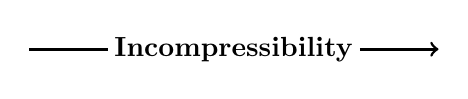
\begin{tikzpicture}
                \draw[-, line width=1pt] (.4,0) -- (1.4,0);
                \node at (3,0) {\textbf{Incompressibility}}; 
                \draw[->, line width=1pt] (4.6,0) -- (5.6,0);
            \end{tikzpicture} \\
        }
        \lfbox[
            border-width=2pt,
            padding-top=0pt,
            padding-bottom=0pt,
            padding-left=-2.5pt,
            padding-right=-2.5pt,
        ]{
            \begin{tikzpicture}
                \draw (0, 0) node[inner sep=0] {
                    \includegraphics*[width=0.25\linewidth]{overoptimization/neg-jpeg-ppo-hartebeest/0.jpg}
                };
                \node[text=black] at (-0.3, 0.6) {\scriptsize \contour{white}{\methodours{}}};
            \end{tikzpicture}
            \hspace{-0.7em}
            \includegraphics*[width=0.25\linewidth]{overoptimization/neg-jpeg-ppo-hartebeest/9.jpg}
            \hspace{-0.7em}
            \includegraphics*[width=0.25\linewidth]{overoptimization/neg-jpeg-ppo-hartebeest/49.jpg}
            \hspace{-0.7em}
            \includegraphics*[width=0.25\linewidth]{overoptimization/neg-jpeg-ppo-hartebeest/69.jpg}
        }
        \vspace{-0.5em} \\
        \lfbox[
            border-width=2pt,
            padding-top=0pt,
            padding-bottom=0pt,
            padding-left=-2.5pt,
            padding-right=-2.5pt,
        ]{
            \begin{tikzpicture}
                \draw (0, 0) node[inner sep=0] {
                    \includegraphics*[width=0.25\linewidth]{overoptimization/neg-jpeg-rwr-zebra/0.jpg}
                };
                \node[text=black] at (-0.4, -0.6) {\scriptsize \contour{white}{\methodrwr{}}};
            \end{tikzpicture}
            \hspace{-0.7em}
            \includegraphics*[width=0.25\linewidth]{overoptimization/neg-jpeg-rwr-zebra/1.jpg}
            \hspace{-0.7em}
            \includegraphics*[width=0.25\linewidth]{overoptimization/neg-jpeg-rwr-zebra/2.jpg}
            \hspace{-0.7em}
            \includegraphics*[width=0.25\linewidth]{overoptimization/neg-jpeg-rwr-zebra/3.jpg}
        }
    \end{minipage}
    }
    \adjustbox{valign=t}{
    \begin{minipage}{0.48\linewidth}
        {
            \centering
            
\begin{tikzpicture}
                \draw[-, line width=1pt, color=white] (0,0) -- (1,0);
                \node at (3,0) {\textbf{Counting Animals}}; 
                \draw[->, line width=1pt, color=white] (4.9,0) -- (5.9,0);
            \end{tikzpicture} \\
        }
        \lfbox[
            border-width=2pt,
            padding-top=0pt,
            padding-bottom=0pt,
            padding-left=-2.5pt,
            padding-right=-8.7pt,
        ]{
            \begin{minipage}{\linewidth}
                \includegraphics*[width=0.25\linewidth]{overoptimization/vlm-counting/six-lions.jpg}
                \hspace{-0.7em}
                \includegraphics*[width=0.25\linewidth]{overoptimization/vlm-counting/seven-birds.jpg}
                \hspace{-0.7em}
                \includegraphics*[width=0.25\linewidth]{overoptimization/vlm-counting/five-wolves.jpg}
                \hspace{-0.7em}
                \includegraphics*[width=0.25\linewidth]{overoptimization/vlm-counting/five-raccoons} \\
                \vspace{-1.2em} \\
                \includegraphics*[width=0.25\linewidth]{overoptimization/vlm-counting/eight-foxes.jpg}
                \hspace{-0.7em}
                \includegraphics*[width=0.25\linewidth]{overoptimization/vlm-counting/three-tigers.jpg}
                \hspace{-0.7em}
                \includegraphics*[width=0.25\linewidth]{overoptimization/vlm-counting/six-turtles.jpg}
                \hspace{-0.7em}
                \includegraphics*[width=0.25\linewidth]{overoptimization/vlm-counting/six-dogs.jpg}
            \end{minipage}
        }
    \end{minipage}
    }
    \caption{
        \textbf{(Reward model overoptimization)}
        Examples of RL overoptimizing reward functions.
        \textbf{(L)}~The diffusion model eventually loses all recognizable semantic content and produces noise when optimizing for incompressibility.
        \textbf{(R)} When optimized for prompts of the form ``$n$ \emph{animals}'', the diffusion model exploits the VLM with a typographic attack \citep{goh2021multimodal}, writing text that is interpreted as the specified number $n$ instead of generating the correct number of animals.
    }
    \label{fig:overoptimization}
\end{figure}

Section~\ref{sec:alg_comparison} highlights the optimization problem: given a reward function, how well can an RL algorithm maximize that reward?
However, finetuning on a reward function, especially a learned one, has been observed to lead to reward overoptimization or exploitation \citep{gao2022overoptimization} in which the model achieves high reward while moving too far away from the pretraining distribution to be useful.

Our setting is no exception, and we provide two examples of reward exploitation in Figure~\ref{fig:overoptimization}.
When optimizing the incompressibility objective, the model eventually stops producing semantically meaningful content, degenerating into high-frequency noise.
Similarly, we observed that LLaVA is susceptible to typographic attacks \citep{goh2021multimodal}.
When optimizing for alignment with respect to prompts of the form ``\emph{$n$ animals}'', \methodours{} exploited deficiencies in the VLM by instead generating text loosely resembling the specified number: for example, ``\emph{sixx ttutttas}'' above a picture of eight turtles.

There is currently no general-purpose method for preventing overoptimization.
One common strategy is to add a KL-regularization term to the reward \citep{ouyang2022instructgpt,stiennon2020feedback}; we refer the reader to the concurrent work of \citet{fan2023dpok} for a study of KL-regularization in the context of finetuning text-to-image diffusion models.
However, \citet{gao2022overoptimization} suggest that existing solutions, including KL-regularization, may be empirically equivalent to early stopping. As a result, in this work, we manually identified the last checkpoint before a model began to deteriorate for each method and used that as the reference for qualitative results.
We highlight this problem as an important area for future work.

\begin{table}[b]
    \centering
    \begin{tabular}{l|c}
        Method & Aesthetic Score \\
        \midrule
        Base model & 5.95 $\pm$ 0.03 \\
        Universal guidance & 6.14 $\pm$ 0.05 \\
        $\text{DDPO}_{\text{IS}}$ @ 20k reward queries & 6.63 $\pm$ 0.03
    \end{tabular}
    \caption{Comparison of DDPO with universal guidance using the LAION aesthetic predictor. We report the mean and one standard error over 50 samples for the prompt ``wolf''.}
    \label{tab:universal_guidance}
\end{table}

\section{Comparison to Classifier Guidance}
Classifier guidance \citep{dhariwal2021diffusion} was originally introduced as a way to improve sample quality for conditional generation using the gradients from an image classifier. For a differentiable reward function such as the LAION aesthetics predictor \citep{schuhmann2022laion}, one could naturally imagine an extension to classifier guidance that uses gradients from such a predictor to improve aesthetic score. The issue is that classifier guidance uses gradients with respect to the noisy images in the intermediate stages of the denoising process, which requires retraining the guidance network on noisy images. Universal guidance \citep{bansal2023universal} sidesteps this issue by applying the guidance network to the fully denoised image predicted by the diffusion model at each step.

We compare DDPO with universal guidance in Table~\ref{tab:universal_guidance}. We used the official implementation of universal guidance\footnote{\url{https://github.com/arpitbansal297/Universal-Guided-Diffusion}} with the recommended hyperparameters for style transfer, substituting the guidance network with the LAION aesthetics predictor. While universal guidance is able to produce a statistically significant improvement in aesthetic score, the change is small compared to DDPO. We only report results averaged over 50 samples for a single prompt, since universal guidance is very slow; on an NVIDIA A100 GPU, it takes almost 2 minutes to generate a single image, whereas standard generation (e.g., from a DDPO-finetuned model) takes 4 seconds.

\section{Comparison to DPOK}
\label{app:dpok}
Here we directly compare our implementation of DDPO to the results reported in the DPOK paper \citep{fan2023dpok}, which was developed concurrently with this work. The key similarities and differences between our experimental setups are summarized below:
\begin{itemize}
    \item For this experiment only, we use Stable Diffusion v1-5 as the base model and train the UNet with low-rank adaptation (LoRA; \cite{hu2021lora}) in order to match DPOK.
    \item Rather than matching the hyperparameters in DPOK, we use the same hyperparameters as in our other experiments (Appendix~\ref{app:hyperparams}) except for the learning rate which we increase to 3e-4. We found that when using LoRA, a higher learning rate is necessary to get comparable performance to full finetuning.
    \item Like DPOK, we train on four prompts: ``a green colored rabbit'' (color), ``four wolves in the park'' (count), ``a dog and a cat'' (composition), and ``a dog on the moon'' (location). Unlike DPOK, we train a single model for all four prompts.
    \item Like DPOK, we train the model using ImageReward \citep{xu2023imagereward} as the reward function. We evaluate the model using ImageReward and the LAION aesthetics predictor \citep{schuhmann2022laion}.
    \item Unlike DPOK, we do not employ KL regularization.
\end{itemize}

\begin{figure}[h!]
    \centering
    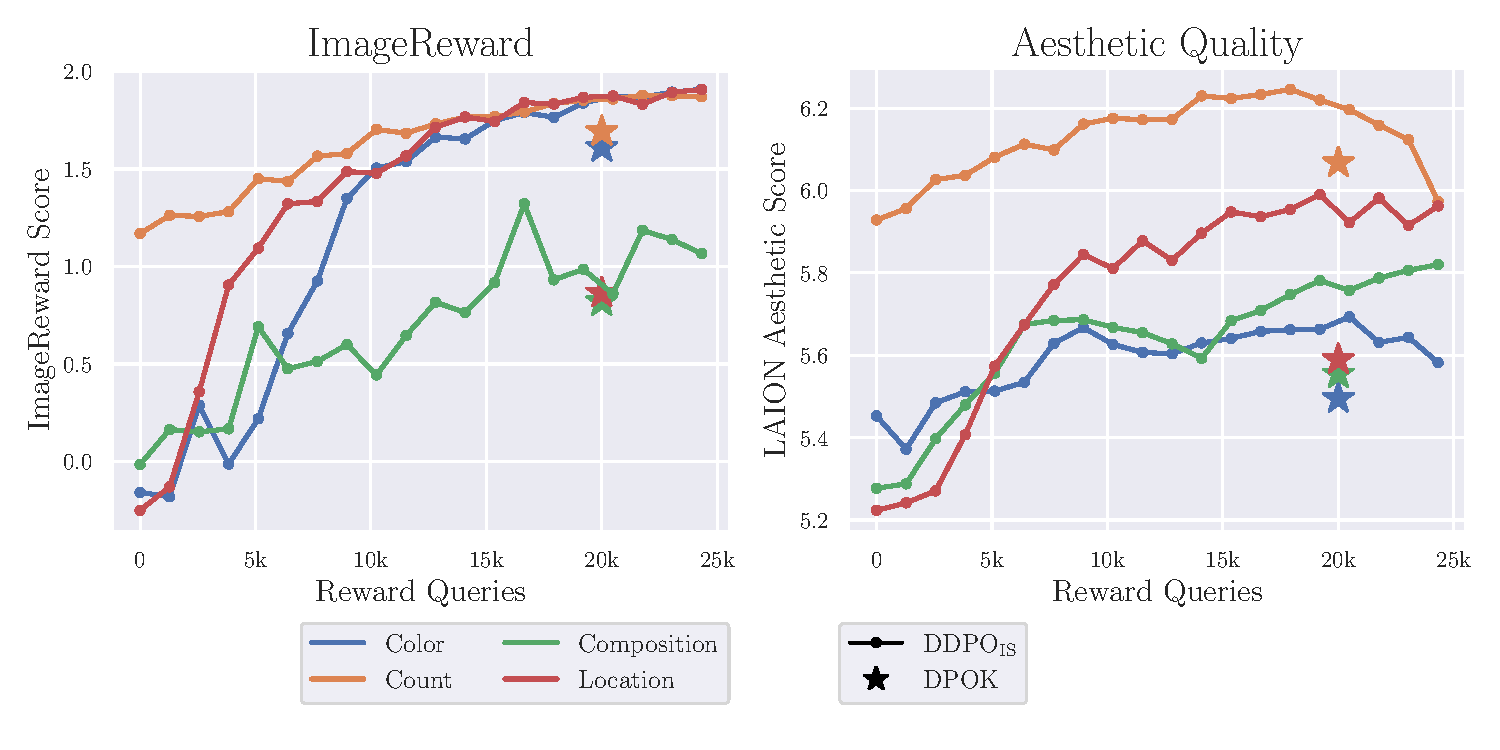
\includegraphics[width=\textwidth]{images/dpok.pdf}
    \caption{Comparison of $\text{DDPO}_\text{IS}$ with DPOK. We take the DPOK numbers directly from the paper, which only reports scores at one point in training (after 20k reward queries). Like in DPOK, scores are averaged over 50 samples for each prompt.}
    \label{fig:dpok_comparison}
\end{figure}

\newpage

The results are presented in Figure~\ref{fig:dpok_comparison}. Our implementation of $\text{DDPO}_\text{IS}$ outperforms DPOK accross the board, without using KL regularization. Figure~\ref{fig:dpok_comparison} also doubles as a quantitative study of overoptimization (Appendix~\ref{app:overoptimization}), since the model is trained with one reward function (ImageReward) and evaluated with another (LAION aesthetic score). We find that significant overoptimization does begin to happen within 25k reward queries for one of the prompts (count: ``four wolves in the park''), which is reflected by a drop in LAION aesthetic score. However, the overoptimization is not severe or unreasonably fast. We provide qualitative samples in Figure~\ref{fig:dpok_qualitative} showing that the model is able to produce high-quality images at 20k reward queries.

\begin{figure}
    \centering
    \begin{minipage}{0.1em}
        \centering
        \vspace{1em}%
        \scriptsize
        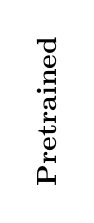
\begin{tikzpicture}
            \node[rotate=90] at (0, 0) {
                \color{black}
                \textbf{Pretrained}
            };
        \end{tikzpicture}
    \end{minipage}%
    \hspace{1em}%
    \begin{minipage}{0.23\linewidth}
        \begin{centering}
            \scriptsize
            \textbf{Color} \\
            \vspace{0.5em}
        \end{centering}
        \lfbox[
            border-width=2pt,
            padding-top=0pt,
            padding-bottom=0pt,
            padding-left=-2.5pt,
            padding-right=-4.8pt,
        ]{
            \begin{minipage}{\linewidth}
                \includegraphics*[width=0.5\linewidth]{dpok/color_before_0.jpg}
                \hspace{-0.7em}
                \includegraphics*[width=0.5\linewidth]{dpok/color_before_1.jpg}
            \end{minipage}
        }
    \end{minipage}
    \hspace{0.1em}%
    \begin{minipage}{0.23\linewidth}
        \begin{centering}
            \scriptsize
            \textbf{Count} \\
            \vspace{0.5em}
        \end{centering}
        \lfbox[
            border-width=2pt,
            padding-top=0pt,
            padding-bottom=0pt,
            padding-left=-2.5pt,
            padding-right=-4.8pt,
        ]{
            \begin{minipage}{\linewidth}
                \includegraphics*[width=0.5\linewidth]{dpok/count_before_0.jpg}
                \hspace{-0.7em}
                \includegraphics*[width=0.5\linewidth]{dpok/count_before_1.jpg}
            \end{minipage}
        }
    \end{minipage}
    \hspace{0.1em}%
    \begin{minipage}{0.23\linewidth}
        \begin{centering}
            \scriptsize
            \textbf{Composition} \\
            \vspace{0.5em}
        \end{centering}
        \lfbox[
            border-width=2pt,
            padding-top=0pt,
            padding-bottom=0pt,
            padding-left=-2.5pt,
            padding-right=-4.8pt,
        ]{
            \begin{minipage}{\linewidth}
                \includegraphics*[width=0.5\linewidth]{dpok/comp_before_0.jpg}
                \hspace{-0.7em}
                \includegraphics*[width=0.5\linewidth]{dpok/comp_before_1.jpg}
            \end{minipage}
        }
    \end{minipage}
    \hspace{0.1em}%
    \begin{minipage}{0.23\linewidth}
        \begin{centering}
            \scriptsize
            \textbf{Location} \\
            \vspace{0.5em}
        \end{centering}
        \lfbox[
            border-width=2pt,
            padding-top=0pt,
            padding-bottom=0pt,
            padding-left=-2.5pt,
            padding-right=-4.8pt,
        ]{
            \begin{minipage}{\linewidth}
                \includegraphics*[width=0.5\linewidth]{dpok/loc_before_0.jpg}
                \hspace{-0.7em}
                \includegraphics*[width=0.5\linewidth]{dpok/loc_before_1.jpg}
            \end{minipage}
        }
    \end{minipage}\\[0.1em]%
    \begin{minipage}{0.1em}
        \centering
        \scriptsize
        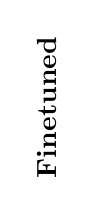
\begin{tikzpicture}
            \node[rotate=90] at (0, 0) {
                \color{black}
                \textbf{Finetuned}
            };
        \end{tikzpicture}
    \end{minipage}%
    \hspace{1em}%
    \begin{minipage}{0.23\linewidth}
        \lfbox[
            border-width=2pt,
            padding-top=0pt,
            padding-bottom=0pt,
            padding-left=-2.5pt,
            padding-right=-4.8pt,
        ]{
            \begin{minipage}{\linewidth}
                \includegraphics*[width=0.5\linewidth]{dpok/color_after_0.jpg}
                \hspace{-0.7em}
                \includegraphics*[width=0.5\linewidth]{dpok/color_after_1.jpg}
            \end{minipage}
        }
    \end{minipage}
    \hspace{0.1em}%
    \begin{minipage}{0.23\linewidth}
        \lfbox[
            border-width=2pt,
            padding-top=0pt,
            padding-bottom=0pt,
            padding-left=-2.5pt,
            padding-right=-4.8pt,
        ]{
            \begin{minipage}{\linewidth}
                \includegraphics*[width=0.5\linewidth]{dpok/count_after_0.jpg}
                \hspace{-0.7em}
                \includegraphics*[width=0.5\linewidth]{dpok/count_after_1.jpg}
            \end{minipage}
        }
    \end{minipage}
    \hspace{0.1em}%
    \begin{minipage}{0.23\linewidth}
        \lfbox[
            border-width=2pt,
            padding-top=0pt,
            padding-bottom=0pt,
            padding-left=-2.5pt,
            padding-right=-4.8pt,
        ]{
            \begin{minipage}{\linewidth}
                \includegraphics*[width=0.5\linewidth]{dpok/comp_after_0.jpg}
                \hspace{-0.7em}
                \includegraphics*[width=0.5\linewidth]{dpok/comp_after_1.jpg}
            \end{minipage}
        }
    \end{minipage}
    \hspace{0.1em}%
    \begin{minipage}{0.23\linewidth}
        \lfbox[
            border-width=2pt,
            padding-top=0pt,
            padding-bottom=0pt,
            padding-left=-2.5pt,
            padding-right=-4.8pt,
        ]{
            \begin{minipage}{\linewidth}
                \includegraphics*[width=0.5\linewidth]{dpok/loc_after_0.jpg}
                \hspace{-0.7em}
                \includegraphics*[width=0.5\linewidth]{dpok/loc_after_1.jpg}
            \end{minipage}
        }
    \end{minipage}%
    \caption{
        Qualtitative examples of the results of ImageReward training on the DPOK prompts: ``a green colored rabbit'' (color), ``four wolves in the park'' (count), ``a dog and a cat'' (composition), and ``a dog on the moon'' (location). The finetuned images are generated from a model trained for 20k reward queries.
    }
    \label{fig:dpok_qualitative}
    \vspace{-15pt}
\end{figure}




\section{Implementation Details}
\label{app:details}

For all experiments, we use Stable Diffusion v1.4 \citep{rombach2022latent} as the base model and finetune only the UNet weights while keeping the text encoder and autoencoder weights frozen.


\subsection{\methodours{} Implementation}
We collect 256 samples per training iteration.
For \methodreinforce, we accumulate gradients across all 256 samples and perform one gradient update.
For \methodppo, we split the samples into 4 minibatches and perform 4 gradient updates.
Gradients are always accumulated across all denoising timesteps for a single sample.
For \methodppo, we use the same clipped surrogate objective as in proximal policy optimization \citep{schulman2017ppo}, but find that we need to use a very small clip range compared to standard RL tasks. We use a clip range of 1e-4 for all experiments.

\subsection{\methodrwr{} Implementation}
We compute the weights for a training iteration using the entire dataset of samples collected for that training iteration.
For $w_\methodrwr$, the weights are computed using the softmax function.
For $w_\sparse$, we use a percentile-based threshold, meaning $C$ is dynamically selected such that the bottom $p$\% of a given pool of samples are discarded and the rest are used for training.

\subsection{Reward Normalization}
In practice, rewards are rarely used as-is, but instead are normalized to have zero mean and unit variance. Furthermore, this normalization can depend on the current state; in the policy gradient context, this is analogous to a value function baseline \citep{sutton1999policy}, and in the RWR context, this is analogous to advantage-weighted regression \citep{peng2019advantage}. In our experiments, we normalize the rewards on a per-context basis. For \methodours, this is implemented as normalization by a running mean and standard deviation that is tracked for each prompt independently. For \methodrwr, this is implemented by computing the softmax over rewards for each prompt independently. For \methodff, this is implemented by computing the percentile-based threshold $C$ for each prompt independently.

\subsection{Resource Details}
\label{app:resources}
\methodrwr{} experiments were conducted on a v3-128 TPU pod, and took approximately 4 hours to reach 50k samples.
\methodours{} experiments were conducted on a v4-64 TPU pod, and took approximately 4 hours to reach 50k samples.
For the VLM-based reward function, LLaVA inference was conducted on a DGX machine with 8 80Gb A100 GPUs.


\subsection{Full Hyperparameters}
\label{app:hyperparams}
\begin{center}
    \begin{tabular}{c|l|c|c|c|c}
        & & \methodppo{} & \methodreinforce{} & \methodrwr{} & \methodff{} \\
        \midrule
        \multirow{2}*{Diffusion} & Denoising steps ($T$) & 50 & 50 & 50 & 50 \\
        & Guidance weight ($w$) & 5.0 & 5.0 & 5.0 & 5.0 \\
        \midrule
        \multirow{7}*{Optimization} & Optimizer & AdamW & AdamW & AdamW & AdamW \\
        & Learning rate & 1e-5 & 1e-5 & 1e-5 & 1e-5 \\
        & Weight decay & 1e-4 & 1e-4 & 1e-4 & 1e-4 \\
        & $\beta_1$ & 0.9 & 0.9 & 0.9 & 0.9 \\
        & $\beta_2$ & 0.999 & 0.999 & 0.999 & 0.999 \\
        & $\epsilon$ & 1e-8 & 1e-8 & 1e-8 & 1e-8 \\
        & Gradient clip norm & 1.0 & 1.0 & 1.0 & 1.0 \\
        \midrule
        \multirow{5}*{\methodrwr} & Inverse temperature ($\beta$) & - & - & 0.2 & - \\
        & Percentile & - & - & - & 0.9 \\
        & Batch size & - & - & 128 & 128 \\
        & Gradient updates per iteration & - & - & 400 & 400 \\ 
        & Samples per iteration & - & - & 10k & 10k \\
        \midrule
        \multirow{4}*{\methodours} & Batch size & 64 & 256 & - & - \\
        & Samples per iteration & 256 & 256 & - & - \\
        & Gradient updates per iteration & 4 & 1 & - & - \\
        & Clip range & 1e-4 & - & - & - \\
    \end{tabular}
\end{center}

\subsection{List of 45 Common Animals}
This list was used for experiments with the aesthetic quality reward function and the VLM-based reward function.
\begin{center}
    \begin{tabular}{c|c|c|c|c|c|c|c|c}
        cat & dog & horse & monkey & rabbit & zebra & spider & bird & sheep \\
        deer & cow & goat & lion & tiger & bear & raccoon & fox & wolf \\
        lizard & beetle & ant & butterfly & fish & shark & whale & dolphin & squirrel \\
        mouse & rat & snake & turtle & frog & chicken & duck & goose & bee \\
        pig & turkey & fly & llama & camel & bat & gorilla & hedgehog & kangaroo
    \end{tabular}
\end{center}

\section{Additional Design Decisions}
\label{app:design}

\subsection{CFG Training}
Recent text-to-image diffusion models rely critically on \emph{classifier-free guidance} (CFG) \citep{ho2021classifierfree} to produce perceptually high-quality results. CFG involves jointly training the diffusion model on conditional and unconditional objectives by randomly masking out the context $\bc$ during training. The conditional and unconditional predictions are then mixed at sampling time using a guidance weight $w$:
\begin{align}
    \tilde{\bm{\epsilon}}_\theta(\bx_t, t, \bc) &= w \bm{\epsilon}_\theta(\bx_t, t, \bc) + (1 - w) \bm{\epsilon}_\theta(\bx_t, t)
\end{align}
where $\bm{\epsilon}_\theta$ is the $\bm{\epsilon}$-prediction parameterization of the diffusion model \citep{ho2020denoising} and $\tilde{\bm{\epsilon}}_\theta$ is the guided $\bm \epsilon$-prediction that is used to compute the next denoised sample.

For reinforcement learning, it does not make sense to train on the unconditional objective since the reward may depend on the context.
However, we found that when only training on the conditional objective, performance rapidly deteriorated after the first round of finetuning. We hypothesized that this is due to the guidance weight becoming miscalibrated each time the model is updated, leading to degraded samples, which in turn impair the next round of finetuning, and so on.
Our solution was to choose a fixed guidance weight and use the guided $\bm{\epsilon}$-prediction during training as well as sampling.
We call this procedure \emph{CFG training}. Figure~\ref{fig:cfg} shows the effect of CFG training on \methodff{}; it has no effect after a single round of finetuning, but becomes essential for subsequent rounds.

\begin{figure}[hbtp]
    \centering
    
\includegraphics[width=0.6\textwidth]{cfg.pdf} \\
    \hspace*{\fill}
    \hspace{4.5em}
    \raisebox{0.14em}{\color{ppo}\rule{1.5em}{0.15em}}
    ~with CFG training
    \hspace{1.5em}
    \raisebox{0.14em}{\color{pg}\rule{1.5em}{0.15em}}
    ~without CFG training
    \hspace*{\fill}
    \caption{
        \textbf{(CFG training)}
        We run the \methodff{} algorithm while optimizing only the conditional $\bm \epsilon$-prediction (\emph{without CFG training}), and while optimizing the guided $\bm \epsilon$-prediction (\emph{with CFG training}).
        Each point denotes a diffusion model update.
        We find that CFG training is essential for methods that do more than one round of interleaved sampling and training.
    } \label{fig:cfg}
\end{figure}

\subsection{Interleaving}
There are two main differences between DDPO and RWR, as compared in Section~\ref{sec:alg_comparison}:
the objective (DDPO uses the policy gradient) and the data distribution (DDPO is significantly more on-policy, collecting 256 samples per iteration as opposed to 10,000 for RWR).
This choice is motivated by standard RL practice, in which policy gradient methods specifically require on-policy data \citep{sutton1999policy}, whereas RWR is designed to work in on off-policy data \citep{nair2020accelerating} and is known to underperform other algorithms in more online settings \citep{duan2016benchmarking}.

However, we can isolate the effect of the data distribution by varying how interleaved the sampling and training are in RWR.
At one extreme is a single-round algorithm \citep{lee2023aligning}, in which $N$ samples are collected from the pretrained model and used for finetuning.
It is also possible to run $k$ rounds of finetuning each on $\frac{N}{k}$ samples collected from the most up-to-date model.
In Figure~\ref{fig:interleaving}, we evaluate this hyperparameter and find that increased interleaving does help up to a point, after which it causes performance degradation. However, RWR is still unable to match the asymptotic performance of DDPO at any level of interleaving.

\begin{figure}
    
\includegraphics[width=\linewidth]{interleave.pdf}
    \caption{
        \textbf{(RWR interleaving ablation)}
        Ablation over the number of samples collected per iteration for RWR. The number of gradient updates per iteration remains the same throughout. We find that more frequent interleaving is beneficial up to a point, after which it causes performance degradation. However, RWR is still unable to match the asymptotic performance of DDPO at any level of interleaving.
    }
    \label{fig:interleaving}
\end{figure}

\section{Quantitative Results for Generalization}
\label{app:generalization}
In Section~\ref{sec:generalization}, we presented qualitative evidence of both the aesthetic quality model and the image-prompt alignment model generalizing to prompts that were unseen during finetuning. In Figure~\ref{fig:quant_generalization}, we provide an additional quantitative analysis of generalization with the aesthetic quality model, where we measure the average reward throughout training for several prompt distributions. In accordance with the qualitative evidence, we see that the model generalizes very well to unseen animals, and everyday objects to a lesser degree.

\begin{figure}
    \centering
    
\includegraphics[width=0.7\linewidth]{aesthetic_quality_generalization.pdf}
    \caption{
        \textbf{(Quantitative generalization)}
        Reward curves demonstrating the generalization of the aesthetic quality objective to prompts not seen during finetuning. The finetuning prompts are a list of 45 common animals, ``unseen animals'' is a list of 38 additional animals, and ``ordinary objects'' is a list of 50 objects (e.g. toaster, chair, coffee cup, etc.).}
    \label{fig:quant_generalization}
\end{figure}

\section{More Samples}
\label{app:more_samples}

Figure~\ref{fig:rwr_samples} shows qualitative samples from the baseline \methodrwr{} method.
Figure~\ref{fig:more-alignment} shows more samples on seen prompts from \methodours{} finetuning with the image-prompt alignment reward function.
Figure~\ref{fig:more-generalization-aesthetic} shows more examples of generalization to unseen animals and everyday objects with the aesthetic quality reward function.
Figure~\ref{fig:more-generalization-alignment} shows more examples of generalization to unseen subjects and activities with the image-prompt alignment reward function.

\begin{figure}
    \centering
    \begin{minipage}{0.48\linewidth}
        \begin{centering}
            \footnotesize 
            \textbf{Pretrained} \\
            \vspace{0.5em}
        \end{centering}
        \lfbox[
            border-width=2pt,
            padding-top=0pt,
            padding-bottom=0pt,
            padding-left=-2.5pt,
            padding-right=-8.5pt,
        ]{
            \begin{minipage}{\linewidth}
                \includegraphics*[width=0.25\linewidth]{algorithm-comparison/pretrained/bird.jpg}
                \hspace{-0.7em}
                \includegraphics*[width=0.25\linewidth]{algorithm-comparison/pretrained/fox.jpg}
                \hspace{-0.7em}
                \includegraphics*[width=0.25\linewidth]{algorithm-comparison/pretrained/bear.jpg}
                \hspace{-0.7em}
                \includegraphics*[width=0.25\linewidth]{algorithm-comparison/pretrained/gorilla.jpg} \\
                \vspace{-1.25em} \\
                \includegraphics*[width=0.25\linewidth]{algorithm-comparison/pretrained/dog.jpg}
                \hspace{-0.7em}
                \includegraphics*[width=0.25\linewidth]{algorithm-comparison/pretrained/hen.jpg}
                \hspace{-0.7em}
                \includegraphics*[width=0.25\linewidth]{algorithm-comparison/pretrained/squirrel.jpg}
                \hspace{-0.7em}
                \includegraphics*[width=0.25\linewidth]{algorithm-comparison/pretrained/cat.jpg}
            \end{minipage}
        }
    \end{minipage}
    \hfill
    \begin{minipage}{0.48\linewidth}
        \begin{centering}
            \footnotesize 
            \textbf{Aesthetic Quality} \\
            \vspace{0.5em}
        \end{centering}
        \lfbox[
            border-width=2pt,
            padding-top=0pt,
            padding-bottom=0pt,
            padding-left=-2.5pt,
            padding-right=-8.5pt,
        ]{
            \begin{minipage}{\linewidth}
                \includegraphics*[width=0.25\linewidth]{algorithm-comparison/aesthetic-rwr/bird.jpg}
                \hspace{-0.7em}
                \includegraphics*[width=0.25\linewidth]{algorithm-comparison/aesthetic-rwr/fox.jpg}
                \hspace{-0.7em}
                \includegraphics*[width=0.25\linewidth]{algorithm-comparison/aesthetic-rwr/bear.jpg}
                \hspace{-0.7em}
                \includegraphics*[width=0.25\linewidth]{algorithm-comparison/aesthetic-rwr/gorilla.jpg} \\
                \vspace{-1.25em} \\
                \includegraphics*[width=0.25\linewidth]{algorithm-comparison/aesthetic-rwr/dog.jpg}
                \hspace{-0.7em}
                \includegraphics*[width=0.25\linewidth]{algorithm-comparison/aesthetic-rwr/hen.jpg}
                \hspace{-0.7em}
                \includegraphics*[width=0.25\linewidth]{algorithm-comparison/aesthetic-rwr/squirrel.jpg}
                \hspace{-0.7em}
                \includegraphics*[width=0.25\linewidth]{algorithm-comparison/aesthetic-rwr/cat.jpg}
            \end{minipage}
        }
    \end{minipage}
    \vspace{0.5em}\\
    \begin{minipage}{0.48\linewidth}
        \begin{centering}
            \footnotesize 
            \textbf{Compressibility} \\
            \vspace{0.5em}
        \end{centering}
        \lfbox[
            border-width=2pt,
            padding-top=0pt,
            padding-bottom=0pt,
            padding-left=-2.5pt,
            padding-right=-8.5pt,
        ]{
            \begin{minipage}{\linewidth}
                \includegraphics*[width=0.25\linewidth]{algorithm-comparison/jpeg-rwr/bird.jpg}
                \hspace{-0.7em}
                \includegraphics*[width=0.25\linewidth]{algorithm-comparison/jpeg-rwr/fox.jpg}
                \hspace{-0.7em}
                \includegraphics*[width=0.25\linewidth]{algorithm-comparison/jpeg-rwr/bear.jpg}
                \hspace{-0.7em}
                \includegraphics*[width=0.25\linewidth]{algorithm-comparison/jpeg-rwr/gorilla.jpg} \\
                \vspace{-1.25em} \\
                \includegraphics*[width=0.25\linewidth]{algorithm-comparison/jpeg-rwr/dog.jpg}
                \hspace{-0.7em}
                \includegraphics*[width=0.25\linewidth]{algorithm-comparison/jpeg-rwr/hen.jpg}
                \hspace{-0.7em}
                \includegraphics*[width=0.25\linewidth]{algorithm-comparison/jpeg-rwr/squirrel.jpg}
                \hspace{-0.7em}
                \includegraphics*[width=0.25\linewidth]{algorithm-comparison/jpeg-rwr/cat.jpg}
            \end{minipage}
        }
    \end{minipage}
    \hfill
    \begin{minipage}{0.48\linewidth}
        \begin{centering}
            \footnotesize 
            \textbf{Incompressibility} \\
            \vspace{0.5em}
        \end{centering}
        \lfbox[
            border-width=2pt,
            padding-top=0pt,
            padding-bottom=0pt,
            padding-left=-2.5pt,
            padding-right=-8.5pt,
        ]{
            \begin{minipage}{\linewidth}
                \includegraphics*[width=0.25\linewidth]{algorithm-comparison/neg-jpeg-rwr/bird.jpg}
                \hspace{-0.7em}
                \includegraphics*[width=0.25\linewidth]{algorithm-comparison/neg-jpeg-rwr/fox.jpg}
                \hspace{-0.7em}
                \includegraphics*[width=0.25\linewidth]{algorithm-comparison/neg-jpeg-rwr/bear.jpg}
                \hspace{-0.7em}
                \includegraphics*[width=0.25\linewidth]{algorithm-comparison/neg-jpeg-rwr/gorilla.jpg} \\
                \vspace{-1.25em} \\
                \includegraphics*[width=0.25\linewidth]{algorithm-comparison/neg-jpeg-rwr/dog.jpg}
                \hspace{-0.7em}
                \includegraphics*[width=0.25\linewidth]{algorithm-comparison/neg-jpeg-rwr/hen.jpg}
                \hspace{-0.7em}
                \includegraphics*[width=0.25\linewidth]{algorithm-comparison/neg-jpeg-rwr/squirrel.jpg}
                \hspace{-0.7em}
                \includegraphics*[width=0.25\linewidth]{algorithm-comparison/neg-jpeg-rwr/cat.jpg}
            \end{minipage}
        }
    \end{minipage} \\
    \caption{
        \textbf{(\methodrwr{} samples)}
    }
    \label{fig:rwr_samples}
\end{figure}


\begin{figure}[t]
    \centering
    \adjustbox{valign=t}{
    \begin{minipage}{0.45\linewidth}
        {
            \centering
            \scriptsize
            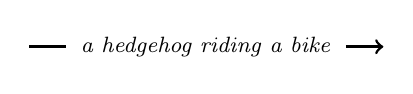
\begin{tikzpicture}
                \draw[-, line width=1pt] (0,.1) -- (0.475,.1);
                \node at (2.25,0.1) {
                    \footnotesize{\emph{a hedgehog riding a bike}}
                };
                \draw[->, line width=1pt] (4.025,.1) -- (4.5,.1);
            \end{tikzpicture} \\
        }
        \lfbox[
            border-width=2pt,
            padding-top=0pt,
            padding-bottom=0pt,
            padding-left=-2.5pt,
            padding-right=-4.8pt,
        ]{
            \begin{minipage}{\linewidth}
                \includegraphics*[width=0.3334\linewidth]{vlm/hedgehog_bike/0.jpg}
                \hspace{-0.6em}
                \includegraphics*[width=0.3334\linewidth]{vlm/hedgehog_bike/1.jpg}
                \hspace{-0.6em}
                \includegraphics*[width=0.3334\linewidth]{vlm/hedgehog_bike/2.jpg}
            \end{minipage}
        }
    \end{minipage}
    }
    \hspace{-.5em}
    \adjustbox{valign=t}{
    \begin{minipage}{0.45\linewidth}
        {
            \centering
            \scriptsize
            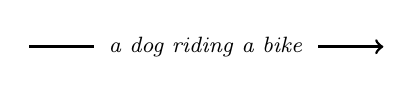
\begin{tikzpicture}
                \draw[-, line width=1pt] (0,.1) -- (0.825,.1);
                \node at (2.25,0.1) {
                    \footnotesize{\emph{a dog riding a bike}}
                };
                \draw[->, line width=1pt] (3.675,.1) -- (4.5,.1);
            \end{tikzpicture} \\
        }
        \lfbox[
            border-width=2pt,
            padding-top=0pt,
            padding-bottom=0pt,
            padding-left=-2.5pt,
            padding-right=-4.8pt,
        ]{
            \begin{minipage}{\linewidth}
                
\includegraphics[width=0.3334\linewidth]{vlm/dog_bike/0.jpg}
                \hspace{-0.6em}
                
\includegraphics[width=0.3334\linewidth]{vlm/dog_bike/2.jpg}
                \hspace{-0.6em}
                
\includegraphics[width=0.3334\linewidth]{vlm/dog_bike/5.jpg}
            \end{minipage}
        }
    \end{minipage}
    } \\
    \vspace{1em}
    \adjustbox{valign=t}{
    \begin{minipage}{0.45\linewidth}
        {
            \centering
            \scriptsize
            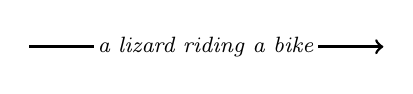
\begin{tikzpicture}
                \draw[-, line width=1pt] (0,.1) -- (0.825,.1);
                \node at (2.25,0.1) {
                    \footnotesize{\emph{a lizard riding a bike}}
                };
                \draw[->, line width=1pt] (3.675,.1) -- (4.5,.1);
            \end{tikzpicture} \\
        }
        \lfbox[
            border-width=2pt,
            padding-top=0pt,
            padding-bottom=0pt,
            padding-left=-2.5pt,
            padding-right=-4.8pt,
        ]{
            \begin{minipage}{\linewidth}
                
\includegraphics[width=0.3334\linewidth]{vlm/lizard_bike/0.jpg}
                \hspace{-0.6em}
                
\includegraphics[width=0.3334\linewidth]{vlm/lizard_bike/1.jpg}
                \hspace{-0.6em}
                
\includegraphics[width=0.3334\linewidth]{vlm/lizard_bike/2.jpg}
            \end{minipage}
        }
    \end{minipage}
    }
    \hspace{-.5em}
    \adjustbox{valign=t}{
    \begin{minipage}{0.45\linewidth}
        {
            \centering
            \scriptsize
            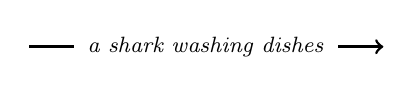
\begin{tikzpicture}
                \draw[-, line width=1pt] (0,.1) -- (0.575,.1);
                \node at (2.25,0.1) {
                    \footnotesize{\emph{a shark washing dishes}}
                };
                \draw[->, line width=1pt] (3.925,.1) -- (4.5,.1);
            \end{tikzpicture} \\
        }
        \lfbox[
            border-width=2pt,
            padding-top=0pt,
            padding-bottom=0pt,
            padding-left=-2.5pt,
            padding-right=-4.8pt,
        ]{
            \begin{minipage}{\linewidth}
                
\includegraphics[width=0.3334\linewidth]{vlm/shark_dishes/0.jpg}
                \hspace{-0.6em}
                
\includegraphics[width=0.3334\linewidth]{vlm/shark_dishes/1.jpg}
                \hspace{-0.6em}
                
\includegraphics[width=0.3334\linewidth]{vlm/shark_dishes/2.jpg}
            \end{minipage}
        }
    \end{minipage}
    } \\
    \vspace{1em}
    \adjustbox{valign=t}{
    \begin{minipage}{0.45\linewidth}
        {
            \centering
            \scriptsize
            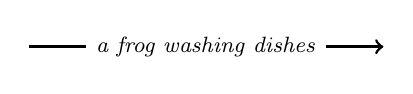
\begin{tikzpicture}
                \draw[-, line width=1pt] (0,.1) -- (0.725,.1);
                \node at (2.25,0.1) {
                    \footnotesize{\emph{a frog washing dishes}}
                };
                \draw[->, line width=1pt] (3.775,.1) -- (4.5,.1);
            \end{tikzpicture} \\
        }
        \lfbox[
            border-width=2pt,
            padding-top=0pt,
            padding-bottom=0pt,
            padding-left=-2.5pt,
            padding-right=-4.8pt,
        ]{
            \begin{minipage}{\linewidth}
                
\includegraphics[width=0.3334\linewidth]{vlm/frog_dishes/0.jpg}
                \hspace{-0.6em}
                
\includegraphics[width=0.3334\linewidth]{vlm/frog_dishes/1.jpg}
                \hspace{-0.6em}
                
\includegraphics[width=0.3334\linewidth]{vlm/frog_dishes/2.jpg}
            \end{minipage}
        }
    \end{minipage}
    }
    \hspace{-.5em}
    \adjustbox{valign=t}{
    \begin{minipage}{0.45\linewidth}
        {
            \centering
            \scriptsize
            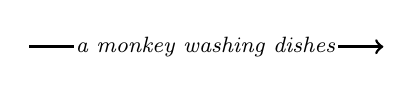
\begin{tikzpicture}
                \draw[-, line width=1pt] (0,.1) -- (0.575,.1);
                \node at (2.25,0.1) {
                    \footnotesize{\emph{a monkey washing dishes}}
                };
                \draw[->, line width=1pt] (3.925,.1) -- (4.5,.1);
            \end{tikzpicture} \\
        }
        \lfbox[
            border-width=2pt,
            padding-top=0pt,
            padding-bottom=0pt,
            padding-left=-2.5pt,
            padding-right=-4.8pt,
        ]{
            \begin{minipage}{\linewidth}
                
\includegraphics[width=0.3334\linewidth]{vlm/monkey_dishes/0.jpg}
                \hspace{-0.6em}
                
\includegraphics[width=0.3334\linewidth]{vlm/monkey_dishes/1.jpg}
                \hspace{-0.6em}
                
\includegraphics[width=0.3334\linewidth]{vlm/monkey_dishes/2.jpg}
            \end{minipage}
        }
    \end{minipage}
    }
    \caption{
        \textbf{(More image-prompt alignment samples)}
    }
    \label{fig:more-alignment}
\end{figure}

\begin{figure}
    \centering
    \begin{minipage}{0.48\linewidth}
        \begin{centering}
            \footnotesize 
            \textbf{Pretrained (New Animals)} \\
            \vspace{0.5em}
        \end{centering}
        \lfbox[
            border-width=2pt,
            padding-top=0pt,
            padding-bottom=0pt,
            padding-left=-2.5pt,
            padding-right=-8.5pt,
        ]{
            \begin{minipage}{\linewidth}
                \includegraphics*[width=0.33\linewidth]{generalization/aesthetic-animal/before/0.jpg}
                \hspace{-0.7em}
                \includegraphics*[width=0.33\linewidth]{generalization/aesthetic-animal/before/1.jpg}
                \hspace{-0.7em}
                \includegraphics*[width=0.33\linewidth]{generalization/aesthetic-animal/before/2.jpg} \\
                \vspace{-1.25em} \\
                \includegraphics*[width=0.33\linewidth]{generalization/aesthetic-animal/before/3.jpg}
                \hspace{-0.7em}
                \includegraphics*[width=0.33\linewidth]{generalization/aesthetic-animal/before/4.jpg}
                \hspace{-0.7em}
                \includegraphics*[width=0.33\linewidth]{generalization/aesthetic-animal/before/5.jpg} \\
                \vspace{-1.25em} \\
                \includegraphics*[width=0.33\linewidth]{generalization/aesthetic-animal/before/6.jpg}
                \hspace{-0.7em}
                \includegraphics*[width=0.33\linewidth]{generalization/aesthetic-animal/before/7.jpg}
                \hspace{-0.7em}
                \includegraphics*[width=0.33\linewidth]{generalization/aesthetic-animal/before/8.jpg}
            \end{minipage}
        }
    \end{minipage}
    \hfill
    \begin{minipage}{0.48\linewidth}
        \begin{centering}
            \footnotesize 
            \textbf{Aesthetic Quality (New Animals)} \\
            \vspace{0.5em}
        \end{centering}
        \lfbox[
            border-width=2pt,
            padding-top=0pt,
            padding-bottom=0pt,
            padding-left=-2.5pt,
            padding-right=-8.5pt,
        ]{
            \begin{minipage}{\linewidth}
                \includegraphics*[width=0.33\linewidth]{generalization/aesthetic-animal/after/0.jpg}
                \hspace{-0.7em}
                \includegraphics*[width=0.33\linewidth]{generalization/aesthetic-animal/after/1.jpg}
                \hspace{-0.7em}
                \includegraphics*[width=0.33\linewidth]{generalization/aesthetic-animal/after/2.jpg} \\
                \vspace{-1.25em} \\
                \includegraphics*[width=0.33\linewidth]{generalization/aesthetic-animal/after/3.jpg}
                \hspace{-0.7em}
                \includegraphics*[width=0.33\linewidth]{generalization/aesthetic-animal/after/4.jpg}
                \hspace{-0.7em}
                \includegraphics*[width=0.33\linewidth]{generalization/aesthetic-animal/after/5.jpg} \\
                \vspace{-1.25em} \\
                \includegraphics*[width=0.33\linewidth]{generalization/aesthetic-animal/after/6.jpg}
                \hspace{-0.7em}
                \includegraphics*[width=0.33\linewidth]{generalization/aesthetic-animal/after/7.jpg}
                \hspace{-0.7em}
                \includegraphics*[width=0.33\linewidth]{generalization/aesthetic-animal/after/8.jpg}
            \end{minipage}
        }
    \end{minipage}
    \vspace{1em}\\
    \begin{minipage}{0.48\linewidth}
        \begin{centering}
            \footnotesize 
            \textbf{Pretrained (Non-Animals)} \\
            \vspace{0.5em}
        \end{centering}
        \lfbox[
            border-width=2pt,
            padding-top=0pt,
            padding-bottom=0pt,
            padding-left=-2.5pt,
            padding-right=-8.5pt,
        ]{
            \begin{minipage}{\linewidth}
                \includegraphics*[width=0.33\linewidth]{generalization/aesthetic-objects/before/0.jpg} 
                \hspace{-0.7em}
                \includegraphics*[width=0.33\linewidth]{generalization/aesthetic-objects/before/1.jpg}
                \hspace{-0.7em}
                \includegraphics*[width=0.33\linewidth]{generalization/aesthetic-objects/before/2.jpg}
                \vspace{-1.25em} \\
                \includegraphics*[width=0.33\linewidth]{generalization/aesthetic-objects/before/3.jpg}
                \hspace{-0.7em}
                \includegraphics*[width=0.33\linewidth]{generalization/aesthetic-objects/before/4.jpg}
                \hspace{-0.7em}
                \includegraphics*[width=0.33\linewidth]{generalization/aesthetic-objects/before/5.jpg}
                \vspace{-1.25em} \\
                \includegraphics*[width=0.33\linewidth]{generalization/aesthetic-objects/before/6.jpg}
                \hspace{-0.7em}
                \includegraphics*[width=0.33\linewidth]{generalization/aesthetic-objects/before/7.jpg}
                \hspace{-0.7em}
                \includegraphics*[width=0.33\linewidth]{generalization/aesthetic-objects/before/8.jpg}
            \end{minipage}
        }
    \end{minipage}
    \hfill
    \begin{minipage}{0.48\linewidth}
        \begin{centering}
            \footnotesize 
            \textbf{Aesthetic Quality (Non-Animals)} \\
            \vspace{0.5em}
        \end{centering}
        \lfbox[
            border-width=2pt,
            padding-top=0pt,
            padding-bottom=0pt,
            padding-left=-2.5pt,
            padding-right=-8.5pt,
        ]{
            \begin{minipage}{\linewidth}
                \includegraphics*[width=0.33\linewidth]{generalization/aesthetic-objects/after/0.jpg} 
                \hspace{-0.7em}
                \includegraphics*[width=0.33\linewidth]{generalization/aesthetic-objects/after/1.jpg}
                \hspace{-0.7em}
                \includegraphics*[width=0.33\linewidth]{generalization/aesthetic-objects/after/2.jpg}
                \vspace{-1.25em} \\
                \includegraphics*[width=0.33\linewidth]{generalization/aesthetic-objects/after/3.jpg}
                \hspace{-0.7em}
                \includegraphics*[width=0.33\linewidth]{generalization/aesthetic-objects/after/4.jpg}
                \hspace{-0.7em}
                \includegraphics*[width=0.33\linewidth]{generalization/aesthetic-objects/after/5.jpg}
                \vspace{-1.25em} \\
                \includegraphics*[width=0.33\linewidth]{generalization/aesthetic-objects/after/6.jpg}
                \hspace{-0.7em}
                \includegraphics*[width=0.33\linewidth]{generalization/aesthetic-objects/after/7.jpg}
                \hspace{-0.7em}
                \includegraphics*[width=0.33\linewidth]{generalization/aesthetic-objects/after/8.jpg}
            \end{minipage}
        }
    \end{minipage} \\
    \caption{
        \textbf{(Aesthetic quality generalization)}
    }
    \label{fig:more-generalization-aesthetic}
\end{figure}


\begin{figure}[t]
    \centering
    \adjustbox{valign=t}{
    \begin{minipage}{0.45\linewidth}
        {
            \centering
            \scriptsize
            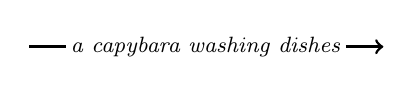
\begin{tikzpicture}
                \draw[-, line width=1pt] (0,.1) -- (0.475,.1);
                \node at (2.25,0.1) {
                    \footnotesize{\emph{a capybara washing dishes}}
                };
                \draw[->, line width=1pt] (4.025,.1) -- (4.5,.1);
            \end{tikzpicture} \\
        }
        \lfbox[
            border-width=2pt,
            padding-top=0pt,
            padding-bottom=0pt,
            padding-left=-2.5pt,
            padding-right=-4.8pt,
        ]{
            \begin{minipage}{\linewidth}
                \includegraphics*[width=0.3334\linewidth]{vlm/capybara_dishes/0.jpg}
                \hspace{-0.6em}
                \includegraphics*[width=0.3334\linewidth]{vlm/capybara_dishes/1.jpg}
                \hspace{-0.6em}
                \includegraphics*[width=0.3334\linewidth]{vlm/capybara_dishes/2.jpg}
            \end{minipage}
        }
    \end{minipage}
    }
    \hspace{-.5em}
    \adjustbox{valign=t}{
    \begin{minipage}{0.45\linewidth}
        {
            \centering
            \scriptsize
            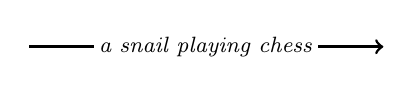
\begin{tikzpicture}
                \draw[-, line width=1pt] (0,.1) -- (0.825,.1);
                \node at (2.25,0.1) {
                    \footnotesize{\emph{a snail playing chess}}
                };
                \draw[->, line width=1pt] (3.675,.1) -- (4.5,.1);
            \end{tikzpicture} \\
        }
        \lfbox[
            border-width=2pt,
            padding-top=0pt,
            padding-bottom=0pt,
            padding-left=-2.5pt,
            padding-right=-4.8pt,
        ]{
            \begin{minipage}{\linewidth}
                
\includegraphics[width=0.3334\linewidth]{vlm/snail_chess/0.jpg}
                \hspace{-0.6em}
                
\includegraphics[width=0.3334\linewidth]{vlm/snail_chess/1.jpg}
                \hspace{-0.6em}
                
\includegraphics[width=0.3334\linewidth]{vlm/snail_chess/5.jpg}
            \end{minipage}
        }
    \end{minipage}
    } \\
    \vspace{1em}
    \adjustbox{valign=t}{
    \begin{minipage}{0.45\linewidth}
        {
            \centering
            \scriptsize
            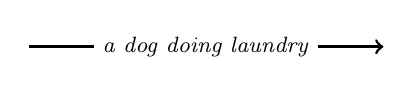
\begin{tikzpicture}
                \draw[-, line width=1pt] (0,.1) -- (0.825,.1);
                \node at (2.25,0.1) {
                    \footnotesize{\emph{a dog doing laundry}}
                };
                \draw[->, line width=1pt] (3.675,.1) -- (4.5,.1);
            \end{tikzpicture} \\
        }
        \lfbox[
            border-width=2pt,
            padding-top=0pt,
            padding-bottom=0pt,
            padding-left=-2.5pt,
            padding-right=-4.8pt,
        ]{
            \begin{minipage}{\linewidth}
                
\includegraphics[width=0.3334\linewidth]{vlm/dog_laundry/0.jpg}
                \hspace{-0.6em}
                
\includegraphics[width=0.3334\linewidth]{vlm/dog_laundry/1.jpg}
                \hspace{-0.6em}
                
\includegraphics[width=0.3334\linewidth]{vlm/dog_laundry/2.jpg}
            \end{minipage}
        }
    \end{minipage}
    }
    \hspace{-.5em}
    \adjustbox{valign=t}{
    \begin{minipage}{0.45\linewidth}
        {
            \centering
            \scriptsize
            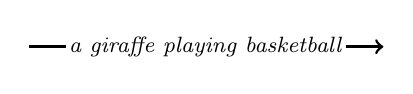
\begin{tikzpicture}
                \draw[-, line width=1pt] (0,.1) -- (0.475,.1);
                \node at (2.25,0.1) {
                    \footnotesize{\emph{a giraffe playing basketball}}
                };
                \draw[->, line width=1pt] (4.025,.1) -- (4.5,.1);
            \end{tikzpicture} \\
        }
        \lfbox[
            border-width=2pt,
            padding-top=0pt,
            padding-bottom=0pt,
            padding-left=-2.5pt,
            padding-right=-4.8pt,
        ]{
            \begin{minipage}{\linewidth}
                
\includegraphics[width=0.3334\linewidth]{vlm/giraffe_basketball/0.jpg}
                \hspace{-0.6em}
                
\includegraphics[width=0.3334\linewidth]{vlm/giraffe_basketball/1.jpg}
                \hspace{-0.6em}
                
\includegraphics[width=0.3334\linewidth]{vlm/giraffe_basketball/2.jpg}
            \end{minipage}
        }
    \end{minipage}
    } \\
    \vspace{1em}
    \adjustbox{valign=t}{
    \begin{minipage}{0.45\linewidth}
        {
            \centering
            \scriptsize
            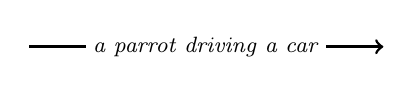
\begin{tikzpicture}
                \draw[-, line width=1pt] (0,.1) -- (0.725,.1);
                \node at (2.25,0.1) {
                    \footnotesize{\emph{a parrot driving a car}}
                };
                \draw[->, line width=1pt] (3.775,.1) -- (4.5,.1);
            \end{tikzpicture} \\
        }
        \lfbox[
            border-width=2pt,
            padding-top=0pt,
            padding-bottom=0pt,
            padding-left=-2.5pt,
            padding-right=-4.8pt,
        ]{
            \begin{minipage}{\linewidth}
                
\includegraphics[width=0.3334\linewidth]{vlm/parrot_car/0.jpg}
                \hspace{-0.6em}
                
\includegraphics[width=0.3334\linewidth]{vlm/parrot_car/1.jpg}
                \hspace{-0.6em}
                
\includegraphics[width=0.3334\linewidth]{vlm/parrot_car/2.jpg}
            \end{minipage}
        }
    \end{minipage}
    }
    \hspace{-.5em}
    \adjustbox{valign=t}{
    \begin{minipage}{0.45\linewidth}
        {
            \centering
            \scriptsize
            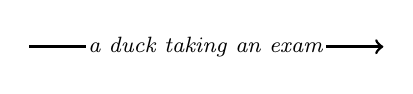
\begin{tikzpicture}
                \draw[-, line width=1pt] (0,.1) -- (0.725,.1);
                \node at (2.25,0.1) {
                    \footnotesize{\emph{a duck taking an exam}}
                };
                \draw[->, line width=1pt] (3.775,.1) -- (4.5,.1);
            \end{tikzpicture} \\
        }
        \lfbox[
            border-width=2pt,
            padding-top=0pt,
            padding-bottom=0pt,
            padding-left=-2.5pt,
            padding-right=-4.8pt,
        ]{
            \begin{minipage}{\linewidth}
                
\includegraphics[width=0.3334\linewidth]{vlm/duck_exam/0.jpg}
                \hspace{-0.6em}
                
\includegraphics[width=0.3334\linewidth]{vlm/duck_exam/1.jpg}
                \hspace{-0.6em}
                
\includegraphics[width=0.3334\linewidth]{vlm/duck_exam/2.jpg}
            \end{minipage}
        }
    \end{minipage}
    } \\
    \vspace{1em}
    \adjustbox{valign=t}{
    \begin{minipage}{0.45\linewidth}
        {
            \centering
            \scriptsize
            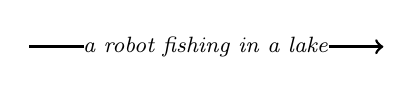
\begin{tikzpicture}
                \draw[-, line width=1pt] (0,.1) -- (0.695,.1);
                \node at (2.25,0.1) {
                    \footnotesize{\emph{a robot fishing in a lake}}
                };
                \draw[->, line width=1pt] (3.805,.1) -- (4.5,.1);
            \end{tikzpicture} \\
        }
        \lfbox[
            border-width=2pt,
            padding-top=0pt,
            padding-bottom=0pt,
            padding-left=-2.5pt,
            padding-right=-4.8pt,
        ]{
            \begin{minipage}{\linewidth}
                
\includegraphics[width=0.3334\linewidth]{vlm/robot_fishing/0.jpg}
                \hspace{-0.6em}
                
\includegraphics[width=0.3334\linewidth]{vlm/robot_fishing/1.jpg}
                \hspace{-0.6em}
                
\includegraphics[width=0.3334\linewidth]{vlm/robot_fishing/2.jpg}
            \end{minipage}
        }
    \end{minipage}
    }
    \hspace{-.5em}
    \adjustbox{valign=t}{
    \begin{minipage}{0.45\linewidth}
        {
            \centering
            \scriptsize
            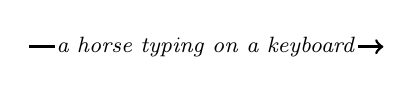
\begin{tikzpicture}
                \draw[-, line width=1pt] (0,.1) -- (0.325,.1);
                \node at (2.25,0.1) {
                    \footnotesize{\emph{a horse typing on a keyboard}}
                };
                \draw[->, line width=1pt] (4.175,.1) -- (4.5,.1);
            \end{tikzpicture} \\
        }
        \lfbox[
            border-width=2pt,
            padding-top=0pt,
            padding-bottom=0pt,
            padding-left=-2.5pt,
            padding-right=-4.8pt,
        ]{
            \begin{minipage}{\linewidth}
                
\includegraphics[width=0.3334\linewidth]{vlm/horse_keyboard/0.jpg}
                \hspace{-0.6em}
                
\includegraphics[width=0.3334\linewidth]{vlm/horse_keyboard/1.jpg}
                \hspace{-0.6em}
                
\includegraphics[width=0.3334\linewidth]{vlm/horse_keyboard/2.jpg}
            \end{minipage}
        }
    \end{minipage}
    } \\
    \vspace{1em}
    \adjustbox{valign=t}{
    \begin{minipage}{0.45\linewidth}
        {
            \centering
            \scriptsize
            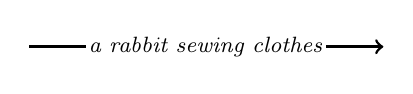
\begin{tikzpicture}
                \draw[-, line width=1pt] (0,.1) -- (0.725,.1);
                \node at (2.25,0.1) {
                    \footnotesize{\emph{a rabbit sewing clothes}}
                };
                \draw[->, line width=1pt] (3.775,.1) -- (4.5,.1);
            \end{tikzpicture} \\
        }
        \lfbox[
            border-width=2pt,
            padding-top=0pt,
            padding-bottom=0pt,
            padding-left=-2.5pt,
            padding-right=-4.8pt,
        ]{
            \begin{minipage}{\linewidth}
                
\includegraphics[width=0.3334\linewidth]{vlm/rabbit_sewing/0.jpg}
                \hspace{-0.6em}
                
\includegraphics[width=0.3334\linewidth]{vlm/rabbit_sewing/1.jpg}
                \hspace{-0.6em}
                
\includegraphics[width=0.3334\linewidth]{vlm/rabbit_sewing/2.jpg}
            \end{minipage}
        }
    \end{minipage}
    }
    \hspace{-.5em}
    \adjustbox{valign=t}{
    \begin{minipage}{0.45\linewidth}
        {
            \centering
            \scriptsize
            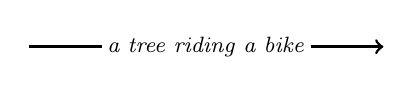
\begin{tikzpicture}
                \draw[-, line width=1pt] (0,.1) -- (0.925,.1);
                \node at (2.25,0.1) {
                    \footnotesize{\emph{a tree riding a bike}}
                };
                \draw[->, line width=1pt] (3.575,.1) -- (4.5,.1);
            \end{tikzpicture} \\
        }
        \lfbox[
            border-width=2pt,
            padding-top=0pt,
            padding-bottom=0pt,
            padding-left=-2.5pt,
            padding-right=-4.8pt,
        ]{
            \begin{minipage}{\linewidth}
                
\includegraphics[width=0.3334\linewidth]{vlm/tree_bike/0.jpg}
                \hspace{-0.6em}
                
\includegraphics[width=0.3334\linewidth]{vlm/tree_bike/1.jpg}
                \hspace{-0.6em}
                
\includegraphics[width=0.3334\linewidth]{vlm/tree_bike/2.jpg}
            \end{minipage}
        }
    \end{minipage}
    } \\
    \vspace{1em}
    \adjustbox{valign=t}{
    \begin{minipage}{0.45\linewidth}
        {
            \centering
            \scriptsize
            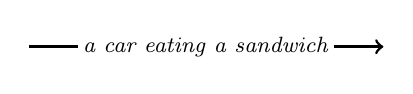
\begin{tikzpicture}
                \draw[-, line width=1pt] (0,.1) -- (0.625,.1);
                \node at (2.25,0.1) {
                    \footnotesize{\emph{a car eating a sandwich}}
                };
                \draw[->, line width=1pt] (3.875,.1) -- (4.5,.1);
            \end{tikzpicture} \\
        }
        \lfbox[
            border-width=2pt,
            padding-top=0pt,
            padding-bottom=0pt,
            padding-left=-2.5pt,
            padding-right=-4.8pt,
        ]{
            \begin{minipage}{\linewidth}
                
\includegraphics[width=0.3334\linewidth]{vlm/car_sandwich/0.jpg}
                \hspace{-0.6em}
                
\includegraphics[width=0.3334\linewidth]{vlm/car_sandwich/1.jpg}
                \hspace{-0.6em}
                
\includegraphics[width=0.3334\linewidth]{vlm/car_sandwich/2.jpg}
            \end{minipage}
        }
    \end{minipage}
    }
    \hspace{-.5em}
    \adjustbox{valign=t}{
    \begin{minipage}{0.45\linewidth}
        {
            \centering
            \scriptsize
            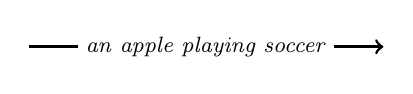
\begin{tikzpicture}
                \draw[-, line width=1pt] (0,.1) -- (0.625,.1);
                \node at (2.25,0.1) {
                    \footnotesize{\emph{an apple playing soccer}}
                };
                \draw[->, line width=1pt] (3.875,.1) -- (4.5,.1);
            \end{tikzpicture} \\
        }
        \lfbox[
            border-width=2pt,
            padding-top=0pt,
            padding-bottom=0pt,
            padding-left=-2.5pt,
            padding-right=-4.8pt,
        ]{
            \begin{minipage}{\linewidth}
                
\includegraphics[width=0.3334\linewidth]{vlm/apple_soccer/0.jpg}
                \hspace{-0.6em}
                
\includegraphics[width=0.3334\linewidth]{vlm/apple_soccer/1.jpg}
                \hspace{-0.6em}
                
\includegraphics[width=0.3334\linewidth]{vlm/apple_soccer/2.jpg}
            \end{minipage}
        }
    \end{minipage}
    }
    \caption{
        \textbf{(Image-prompt alignment generalization)}
    }
    \label{fig:more-generalization-alignment}
\end{figure}

\end{appendices}